%% LyX 2.3.6.1 created this file.  For more info, see http://www.lyx.org/.
%% Do not edit unless you really know what you are doing.
\documentclass[english]{article}
\usepackage[T1]{fontenc}
\usepackage[latin9]{inputenc}
\usepackage{geometry}
\geometry{verbose,tmargin=2.5cm,bmargin=2.5cm,lmargin=2.5cm,rmargin=2.5cm}
\usepackage{array}
\usepackage{fancybox}
\usepackage{calc}
\usepackage{amsmath}
\usepackage{graphicx}
\PassOptionsToPackage{normalem}{ulem}
\usepackage{ulem}

\makeatletter

%%%%%%%%%%%%%%%%%%%%%%%%%%%%%% LyX specific LaTeX commands.
%% Because html converters don't know tabularnewline
\providecommand{\tabularnewline}{\\}

\makeatother

\usepackage{babel}
\begin{document}
{[}SPLIT\_HERE{]}
\begin{enumerate}
\item \textbf{{[}ALVL/9597/2015/P1/Q1{]} }

The file \texttt{ADMISSIONS-DATA.TXT} contains the daily total admissions
to a theme park over a period of 50 days. 

The task is to read the numbers from the file and display a sorted
list. 

You will program two different sort algorithms: 
\begin{enumerate}
\item A bubble sort. 
\item Either a quick sort or an insertion sort but not both. 
\end{enumerate}
Task 1.1

Write code for a procedure to display a menu with the following options: 
\begin{center}
\noindent\ovalbox{\begin{minipage}[t]{1\columnwidth - 2\fboxsep - 0.8pt}%
\begin{enumerate}
\item[1]  Read file data
\item[2] Bubble sort
\item[3] Quick sort/ Insertion sort
\item[4] End Task
\end{enumerate}
%
\end{minipage}}
\par\end{center}

\subsubsection*{Task 1.2}

Write the program code for a procedure to implement menu option 1.

\subsubsection*{Evidence 1}
\begin{itemize}
\item The program code for the menu. 
\item Program code for menu option 1. \hfill{}{[}5{]} 
\end{itemize}
Options 2 and 3 will sort and display the sorted data. The algorithm
for a bubble sort is given in file \texttt{BUBBLE.TXT}. 

Write program code as a procedure to implement the bubble sort. 

\subsubsection*{Evidence 2}
\begin{itemize}
\item The bubble sort code procedure. \hfill{}{[}1{]}
\end{itemize}
Write program code as a procedure to implement the quick sort or the
insertion sort. 

\subsubsection*{Evidence 3}
\begin{itemize}
\item Indicate the sort method used.
\item The program for the sort method used. \hfill{}{[}4{]}
\end{itemize}


\subsubsection*{Task 1.3}

Additional code is to be written for each sort procedure. The sort
methods will count and display the number of comparisons made in completing
the sort process. This will provide an indicator of the efficiency
of each algorithm.

Write the additional code to count and display the number of comparisons
made for each sort method.

\subsubsection*{Evidence 4}
\begin{itemize}
\item The output from menu option 2. \hfill{} {[}2{]}
\end{itemize}

\subsubsection*{Evidence 5}
\begin{itemize}
\item The output from menu option 3. \hfill{} {[}2{]}
\end{itemize}
{[}SPLIT\_HERE{]}
\item \textbf{{[}ALVL/9597/2015/P1/Q2{]} }

The pseudocode procedure below is given a denary number. The procedure
then outputs the binary equivalent of the denary number.

\noindent %
\noindent\begin{minipage}[t]{1\columnwidth}%
\texttt{PROCEDURE Converter(DenaryNumber : INTEGER) }

\texttt{\qquad{}IF DenaryNumber = 0 OR DenaryNumber = 1 }

\texttt{\qquad{}\qquad{}THEN }

\texttt{\qquad{}\qquad{}\qquad{}OUTPUT DenaryNumber }

\texttt{\qquad{}\qquad{}ELSE }

\texttt{\qquad{}\qquad{}\qquad{}OUTPUT DenaryNumber MOD 2 }

\texttt{\qquad{}\qquad{}\qquad{}Converter(DenaryNumber DIV 2) }

\texttt{\qquad{}ENDIF }

\texttt{ENDPROCEDURE}%
\end{minipage}

\subsubsection*{Task 2.1}

Write program code to implement the given procedure. 

Execute the procedure using 56 as the parameter. 

\subsubsection*{Evidence 6}
\begin{itemize}
\item Program code. 
\item Screenshot showing the output. \hfill{}{[}6{]}
\end{itemize}

\subsubsection*{Task 2.2}

There is an error with the given algorithm. 

Describe the error and the effect it created on the output in Evidence
6. 

\subsubsection*{Evidence 7}
\begin{itemize}
\item Statement(s) to answer Task 2.2. \hfill{}{[}1{]}
\end{itemize}

\subsubsection*{Task 2.3}

Make changes to the procedure Converter which will correct the error. 

Draw up a list of test cases for the testing of the amended code.
by completing a table with the following headings: 
\begin{center}
\begin{tabular}{|l|l|l|}
\hline 
\texttt{DenaryNumber} & Purpose of the test & Expected output\tabularnewline
\hline 
 &  & \tabularnewline
\hline 
$\vdots$ & $\vdots$ & $\vdots$\tabularnewline
\hline 
 &  & \tabularnewline
\hline 
\end{tabular}
\par\end{center}

\subsubsection*{Evidence 8}
\begin{itemize}
\item The amended PROCEDURE Converter program code.
\item The completed table. 
\item Screenshots for two of the tests. \hfill{}{[}11{]}
\end{itemize}
{[}SPLIT\_HERE{]}
\item \textbf{{[}ALVL/9597/2015/P1/Q3{]} }

When buying software. the purchaser is issued with a licence key.
The product licence can be purchased for either one or three computers.
A file is maintained of all the licence keys currently active and
whether the licence was for a single-user or 3-users.

The licence key is a 10 character code as follows: 
\begin{center}
\texttt{CCCCCCCCCD }
\par\end{center}
\begin{itemize}
\item \texttt{C} = a randomly generated uppercase letter. 
\item \texttt{D} = a check digit character calculated from the preceding
nine letters.
\end{itemize}
A new licence key is generated for each purchase. 

An example key is produced as follows: 
\begin{itemize}
\item randomly generated letters: \texttt{FGKWRDFTA} 
\item a set of products is calculated as shown: 
\begin{center}
\begin{tabular}{|>{\centering}p{0.1\columnwidth}|>{\centering}p{0.1\columnwidth}|c|c|}
\hline 
Randomly generated letter & ASCII code & Multiplier & Product\tabularnewline
\hline 
\texttt{F} & 70 & 1 & 70\tabularnewline
\hline 
\texttt{G} & 71 & 2 & 142\tabularnewline
\hline 
\texttt{K} & 75 & 3 & 225\tabularnewline
\hline 
\texttt{W} & 87 & 4 & 348\tabularnewline
\hline 
\texttt{R} & 82 & 5 & 410\tabularnewline
\hline 
\texttt{D} & 68 & 6 & 408\tabularnewline
\hline 
\texttt{F} & 70 & 7 & 490\tabularnewline
\hline 
\texttt{T} & 84 & 8 & 672\tabularnewline
\hline 
\texttt{A} & 65 & 9 & 585\tabularnewline
\hline 
\end{tabular}
\par\end{center}
\item Then the total of the products is calculated:
\begin{center}
\begin{tabular}{|c|c|}
\hline 
Total & 3350\tabularnewline
\hline 
\end{tabular}
\par\end{center}
\item The total 3350 is then divided by 11 to give remainder 6. which becomes
the check digit character. 
\item This gives the complete licence key: \texttt{FGKWRDFTA6 }
\item If the calculation gives remainder 10, the check digit character used
is \texttt{X}.
\end{itemize}

\subsubsection*{Task 3.1}

Design a function \texttt{LicenceKey} to generate a new licence key. 

Write program code to implement the function. 

Test the function for \textbf{three} new licence keys. 

\subsubsection*{Evidence 9}
\begin{itemize}
\item Program code for the \texttt{LicenceKey} function. 
\item Screenshot(s) showing the generation of the three new licence keys.
\hfill{}{[}10{]}
\end{itemize}

\subsubsection*{Task 3.2}

A file \texttt{LICENCE-KEYS.TXT} is maintained storing all licence
keys which are currently active. This test file has 20 licence records.You
will need this file for the programming which follows. 

Typical data for two licences are shown: 

\texttt{SYNCTKMMF8 1}

indicates this is a single-user licence. 

\texttt{SNPHHUATV7 3 1} 

purchased as a 3-user licence. but currently has only one registered
user. 

Write program code for a menu with the following options: 
\begin{center}
\noindent\ovalbox{\begin{minipage}[t]{1\columnwidth - 2\fboxsep - 0.8pt}%
\begin{enumerate}
\item[1]  Purchase of a new licence for either a single-user or a 3-user licence
\item[2] Register an additional user to an active 3-user licence
\item[3] End
\end{enumerate}
%
\end{minipage}}
\par\end{center}

\subsubsection*{Task 3.3}

Write code as a procedure for menu option 1.

The requirement will be: 
\begin{itemize}
\item input from the user the type of licence.
\item Generate the new licence key. 
\item Display licence key issued.
\item Save the data as a new record in the \texttt{LICENCE-KEYS.TXT} file. 
\item Display final contents of \texttt{LICENCE-KEYS.TXT} file. 
\end{itemize}

\subsubsection*{Evidence 10}
\begin{itemize}
\item Program code for menu option 1. 
\item Screenshot(s). showing evidence for the issue of the two types of
licence, displaying: 
\begin{itemize}
\item the licence key issued 
\item the final contents of \texttt{LICENCE-KEYS.TXT} file. \hfill{}{[}6{]}
\end{itemize}
\end{itemize}

\subsubsection*{Task 3.4}

Program menu option 2.

Carry out three relevant tests.

\subsubsection*{Evidence 11}
\begin{itemize}
\item Program code for menu option 2.
\item Screenshot evidence of three test cases. \hfill{}{[}5{]}
\end{itemize}
When a licence is purchased, the licence key, licence type (single-user
or 3-user), purchase date and name of the purchaser are recorded. 

A registration process then follows for each computer. 
\begin{itemize}
\item The computer to which a licence is registered has its MAC address
and the date of registration recorded. 
\end{itemize}
The program design to manage purchases and registrations is to be
implemented with object-oriented programming with the following three
classes: 
\begin{center}
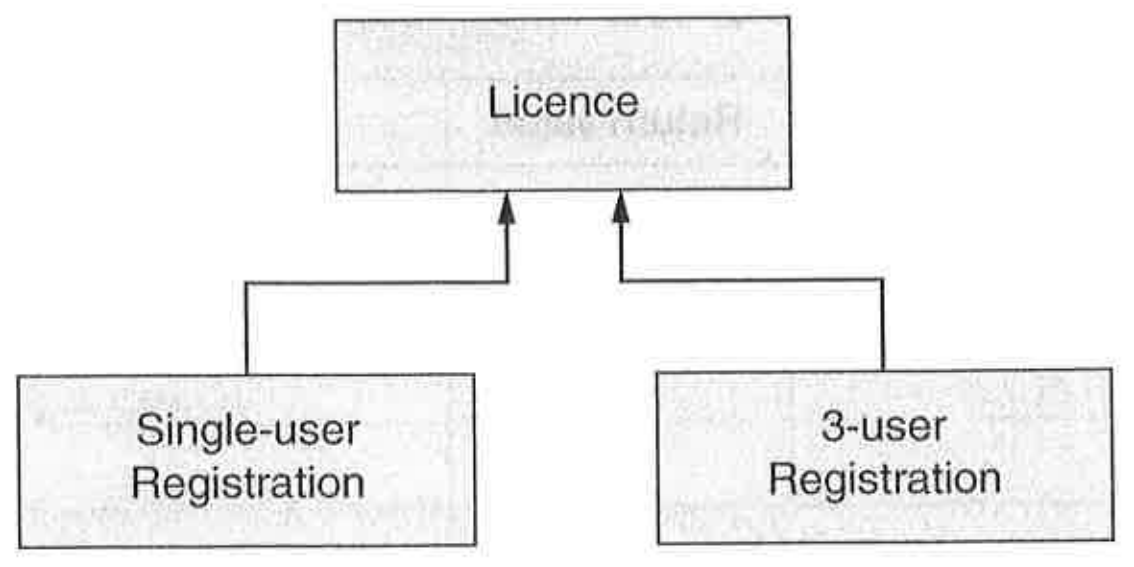
\includegraphics[width=0.5\paperwidth]{C:/Users/Admin/Desktop/Github/question_bank/LyX/static/img/9597-ALVL-2015-P1-Q3}
\par\end{center}

\subsubsection*{Task 3.5}

Write program code \textbf{only} for the three classes shown. 

Do not attempt to develop the application further.

\subsubsection*{Evidence 12}
\begin{itemize}
\item Program code for the three classes.\hfill{}{[}9{]}
\end{itemize}
{[}SPLIT\_HERE{]}
\item \textbf{{[}ALVL/9597/2015/P1/Q4{]} }

Users of a local area network each have a network account ID. The
IDs have the format 2015\_NNNN. where N is a digit. 

\subsubsection*{Task 4.1}

Complete the test case table with the addition of \textbf{three} more
invalid User IDs. The reasons for their invalidity should be different. 

The return value is a code as follows: 
\begin{itemize}
\item 0 - valid User lD 
\item 1 - the User ID was not 9 characters 
\item you will use other integer numbers for other invalid cases. 
\begin{center}
\begin{tabular}{|>{\centering}p{0.1\columnwidth}|>{\centering}p{0.1\columnwidth}|c|c|}
\hline 
Test Number & User ID & Return value & Explanation of the test case\tabularnewline
\hline 
1 & \texttt{2015\_0987} & \texttt{0} & Valid User ID\tabularnewline
\hline 
2 &  &  & \tabularnewline
\hline 
3 &  &  & \tabularnewline
\hline 
4 &  &  & \tabularnewline
\hline 
\end{tabular}
\par\end{center}

\end{itemize}
\hfill{}{[}10{]}

\subsubsection*{Evidence 13}
\begin{itemize}
\item The completed test case table. \hfill{}{[}6{]}
\end{itemize}

\subsubsection*{Task 4.2}

Write program code for a function to validate a User ID. The function
header has the format: 
\begin{center}
\texttt{FUNCTION ValidateUserID (ThisUserID : STRING) RETURNS INTEGER }
\par\end{center}

Write a program to:
\begin{itemize}
\item Input an ID entered by the user 
\item Validate the input using the function\texttt{ ValidateUserID }
\item Output a message describing the validity of the input. 
\end{itemize}
\hfill{}{[}10{]}

\subsubsection*{Evidence 14}
\begin{itemize}
\item Program code for the function \texttt{ValidateUserID} \hfill{}{[}4{]}
\item \textbf{Three} screenshots showing the testing of Test Numbers 2,
3, and 4. \hfill{}{[}3{]}
\end{itemize}
You are to design an object-oriented program which simulates a print
queue for a printer on a local area network (LAN).The print queue
consists at any time of none, one, or more print jobs. 

Each user can send a print job from any of the terminals on the LAN.
Each terminal on the network is identified by an integer number in
the range 1 to 172. 

The program you are to design will record for each printjob: 
\begin{itemize}
\item the user lD
\item the terminal number from which the print request was sent
\item the file size (integer in Kbytes).
\end{itemize}
In practice, there are several print queues each associated with a
different printer. Each printer is identified by a short name, such
as \texttt{Room16}. 

Task 4.3

Design and write program code to define one or more classes and other
appropriate data structures for this application. 

\subsubsection*{Evidence 15}

Program code for the class(es). \hfill{}{[}6{]} 

A print queue behaves as a queue data structure. 

Assume, for testing purposes: 
\begin{itemize}
\item there is a single printer on the LAN 
\item the maximum print queue size for the printer is five print jobs. 
\end{itemize}
The main program will simulate: 
\begin{itemize}
\item the sending of print jobs to the printer by different users 
\begin{itemize}
\item that is, the addition of a print job to the print queue 
\end{itemize}
\item the output of a job from the print queue 
\begin{itemize}
\item that is, the removal of a print job from the print queue 
\end{itemize}
\end{itemize}
The program design has the following menu: 
\begin{center}
\noindent\ovalbox{\begin{minipage}[t]{1\columnwidth - 2\fboxsep - 0.8pt}%
\begin{enumerate}
\item[1]  New print job added to print queue 
\item[2] Next print job output from printer
\item[3] Current print queue displayed
\item[4] End
\end{enumerate}
%
\end{minipage}}
\par\end{center}

The program simulates the working of the print queue as follows: 
\begin{enumerate}
\item[1.] The empty print queue is initialised. 
\item[2.]  The program user selects menu options 1, 2 and 3 in any order. 
\item[3.]  The program user selects menu opt\textbf{two}ion 4.
\end{enumerate}

\subsubsection*{Task 4.4}

Write program code to: 
\begin{itemize}
\item display the main menu 
\item input the choice by the user 
\item run the appropriate code for the choice made.
\end{itemize}

\subsubsection*{Evidence 16}

The program code. \hfill{}{[}3{]}

\subsubsection*{Task 4.5}

Write program code to initialise the print queue for the \texttt{Room16}
printer. 

Write program code to display the current state of the print queue.

\subsubsection*{Evidence 17}

The program code for:
\begin{itemize}
\item initialising the print queue
\item output of the current print queue. \hfill{}{[}6{]}
\end{itemize}

\subsubsection*{Task 4.6}

Write program code to add a new print job to the print queue.

The requirement will be:
\begin{itemize}
\item program user enters data for the new print job
\item print job is added to the print queue.
\end{itemize}
Test the code by adding one new print job.

\subsubsection*{Evidence 18}
\begin{itemize}
\item Program code to add a new print job.
\item Screenshot following menu option 1 then menu option 3. \hfill{}{[}4{]}
\end{itemize}

\subsubsection*{Task 4.7}

Write program code to output the next print job from the printer.

This code will execute from menu option 2.

Test the code by:
\begin{itemize}
\item adding three print jobs
\item outputting the next print job.
\end{itemize}

\subsubsection*{Evidence 19}
\begin{itemize}
\item Program code to output next print job.
\item Screenshot following menu option 1 three times. then menu option 2,
and menu option 3. \hfill{}{[}6{]}
\end{itemize}
{[}SPLIT\_HERE{]}
\item \textbf{{[}ALVL/9597/2015/P2/Q1{]} }

The management of a university is keen to implement changes which
will result in higher student attainment. The management believes
this is possible if it collects more data about its students which
is then analysed.

Possible data that might be collected includes: assignment grades,
books taken out of the library, attendance at lectures, attendance
at tutorials, meetings with personal tutor, email exchanges with university
staff. and participation in sporting and cultural activities.

University staff are classified as either academic or management.
All data about students will be available to academic staff for viewing
and editing. Summary information, which does not identify any individual
student. will be viewable by some management staff. Students have
no access to the data.

A project working party is to be set up consisting of representatives
from across the university. The working party will define the scope
of the project. It will consider what data is to be collected. it
will also decide what the data is to be used for and consider any
potential further use of the data.

If this project has a successful outcome, the university will market
its expertise to other universities. 
\begin{enumerate}
\item Give \textbf{three} different representative members of the working
party. Justify each choice. \hfill{}{[}6{]}
\item The working party has been asked to produce a list of issues that
will be considered by the Ethics Committee of the university.

State \textbf{two} issues that could be on the list.\hfill{} {[}2{]}
\end{enumerate}
After consideration of the reports from the working party and the
Ethics Committee the university management decide to proceed with
the project. A project team is put together to design and implement
a new software system.

The initial work of the project team involves an investigation process. 
\begin{enumerate}
\item[(c)] Name \textbf{two }techniques that can be used by the project team
in the investigation process. For each technique, explain how it can
be used in this project.\hfill{} {[}6{]}
\item[(d)] A detailed report is produced following the investigation.Thls report
will form the starting point of the design stage. Describe \textbf{two}
sections of the report.\hfill{} {[}4{]}
\end{enumerate}
The project team draw up a list of activities that will be required
for the completion of the software project:
\begin{center}
\begin{tabular}{|c|l|c|}
\hline 
Activity & \texttt{\hspace{0.01\columnwidth}}Activity Description  & Expected Duration (in weeks)\tabularnewline
\hline 
A & Design solution to project & 10\tabularnewline
\hline 
B & Development of solution to project & 25\tabularnewline
\hline 
C & Produce documentation & 12\tabularnewline
\hline 
D & Testing & 30\tabularnewline
\hline 
E & implement system & 8\tabularnewline
\hline 
F & Acceptance trials & 2\tabularnewline
\hline 
\end{tabular}
\par\end{center}

A first attempt to produce a Program Evaluation and Review Technique
(PERT) chart from the activity table is: 
\begin{center}
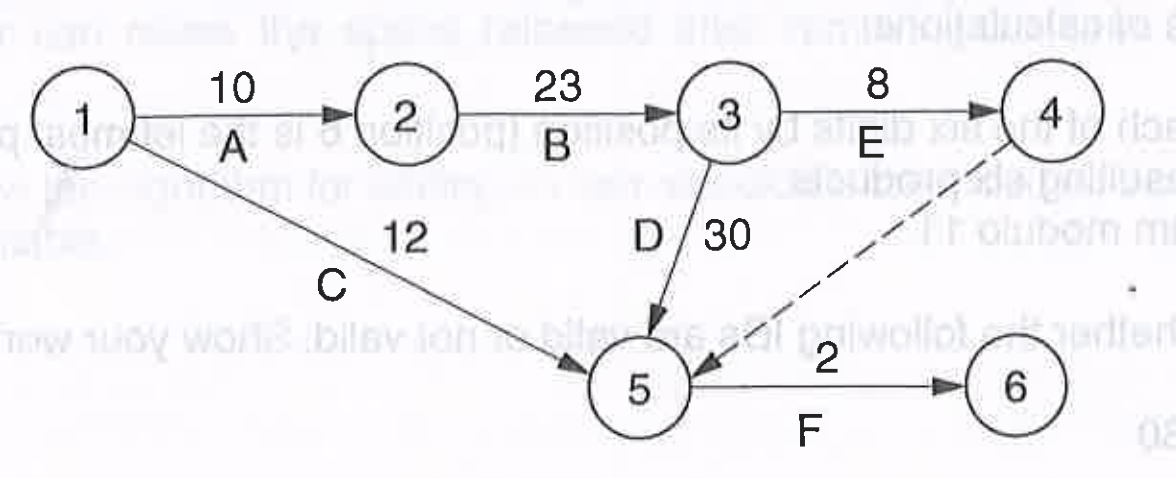
\includegraphics[width=0.5\paperwidth]{C:/Users/Admin/Desktop/Github/question_bank/LyX/static/img/9597-ALVL-2015-P2-Q1}
\par\end{center}
\begin{enumerate}
\item[(e)] {}
\begin{enumerate}
\item Describe \textbf{two} benefits that can be gained by producing a PERT
chart from the activity table. \hfill{}{[}2{]}
\item Explain the significance of the dashed line on the PERT chart. \hfill{}{[}2{]}
\item There are two errors on the PERT chart. identify these errors. Redraw
the PERT chart to show the changes needed to correct these errors.
\hfill{}{[}2{]}
\end{enumerate}
\item[(f)]  Using your PERT chart from part \textbf{(e)(iii)}: 
\begin{itemize}
\item State the minimum time in which the project could be completed.\hfill{}
{[}1{]}
\item By how many weeks can the start of the production of documentation
be delayed without delaying the whole project? \hfill{}{[}1{]}
\item Describe and give an example of concurrent activities.\hfill{} {[}2{]}
\item Describe and give an example of dependent activities. \hfill{}{[}2{]}
\end{itemize}
\end{enumerate}
Output from the system is made available to permitted staff via the
university intranet. However, the university intranet can be accessed
by all students and staff. both locally and remotely, via the lnternet.
The system needs security measures to prevent all types of unauthorised
access. 
\begin{enumerate}
\item[(g)]  Describe\textbf{ two} suitable physical security measures that could
be adopted. \hfill{}{[}4{]}
\item[(h)]  Describe \textbf{two} suitable software security measures that could
be adopted. \hfill{}{[}4{]}
\end{enumerate}
Following the success of the project, management decides that the
software system will be marketed to other universities. 
\begin{enumerate}
\item[(i)]  Explain how the university's investment in the software can be legally
protected. \hfill{}{[}2{]}
\end{enumerate}
{[}SPLIT\_HERE{]}
\item \textbf{{[}ALVL/9597/2015/P2/Q2{]} }

A stock control system requires that each stock item has a unique
ID consisting of six digits. The sixth digit is a check digit. This
check digit ensures that a value of 0 is the final result of the following
series of calculations:
\begin{itemize}
\item multiply each of the six digits by its position (position 6 is the
leftmost position)
\item sum the resulting six products
\item find the sum modulo 11.
\end{itemize}
\begin{enumerate}
\item Deduce whether the following IDs are valid or not valid. Show your
working. 
\begin{enumerate}
\item 810230 \hfill{}{[}2{]}
\item 371025 \hfill{}{[}2{]}
\end{enumerate}
\item The ID 483095 is a valid lD. Describe \textbf{one} typical data entry
error for this ID. Show how this error would be detected.\hfill{}
{[}3{]}
\item Describe a method of verification that can be used when an ID is entered
from a data entry form.\hfill{} {[}3{]}
\end{enumerate}
{[}SPLIT\_HERE{]}
\item \textbf{{[}ALVL/9597/2015/P2/Q3{]} }

A simple queue data structure is implemented using a one-dimensional
array and two pointers, Head and Tail, as shown:
\begin{center}
\begin{tabular}{r|l|l}
\multicolumn{1}{r}{} & \multicolumn{1}{l}{\texttt{Queue}} & \tabularnewline
\cline{2-2} 
\texttt{1} & \texttt{Mac} & \tabularnewline
\cline{2-2} 
\texttt{2} & \texttt{Ben} & $\impliedby$ \texttt{Head}\tabularnewline
\cline{2-2} 
\texttt{3} & \texttt{Dog} & \tabularnewline
\cline{2-2} 
\texttt{4} & \texttt{Can} & \tabularnewline
\cline{2-2} 
\texttt{5} & \texttt{Yog} & \tabularnewline
\cline{2-2} 
\texttt{6} & \texttt{Hur} & \tabularnewline
\cline{2-2} 
\texttt{7} &  & $\impliedby$ \texttt{Tail}\tabularnewline
\cline{2-2} 
\texttt{8} &  & \tabularnewline
\cline{2-2} 
\texttt{9} &  & \tabularnewline
\cline{2-2} 
\texttt{10} &  & \tabularnewline
\cline{2-2} 
\end{tabular}
\par\end{center}
\begin{enumerate}
\item Show the state of the above queue after: 
\begin{itemize}
\item two items, Dap and Eck, are added (in that order) 
\item one item is removed. \hfill{}{[}3{]}
\end{itemize}
When ten items have been added, this simple queue cannot accept any
further items. 
\item A first attempt at an algorithm for adding an item to this queue is:

\noindent\begin{minipage}[t]{1\columnwidth}%
\texttt{01 IF ..............................}

\texttt{02 \qquad{}THEN }

\texttt{03 \qquad{}\qquad{}OUTPUT \textquotedbl No more room to
add items\textquotedblright{} }

\texttt{04 \qquad{}ELSE }

\texttt{05 \qquad{}\qquad{}INPUT \textquotedbl New item to be added\textquotedbl ,
NewItem }

\texttt{06 \qquad{}\qquad{}Queue{[}..............................{]}
<- NewItem }

\texttt{O7 \qquad{}\qquad{}.............................. }

\texttt{O8 ENDIF }%
\end{minipage}

Write the pseudocode to show the completed lines 01, 06, and 07. \hfill{}{[}3{]}
\item Give the initial value for \texttt{Tail} when the queue is created
and justify your answer. \hfill{}{[}2{]}
\end{enumerate}
The programmer can reuse the space released after removing an item.
This maximises the available space.
\begin{enumerate}
\item[(d)]  Describe how the algorithm for adding an item should be amended
so that the released space is made available. \hfill{}{[}2{]}
\end{enumerate}
{[}SPLIT\_HERE{]}
\item \textbf{{[}ALVL/9597/2015/P2/Q4{]} }

An algorithm for converting a number n from denary to octal uses the
three built-in functions: 
\begin{center}
\begin{tabular}{|l|>{\raggedright}p{0.15\columnwidth}|>{\raggedright}p{0.25\columnwidth}|}
\hline 
\texttt{\hspace{0.01\columnwidth}}Function & \texttt{\hspace{0.01\columnwidth}}Description & \texttt{\hspace{0.01\columnwidth}}Example\tabularnewline
\hline 
\texttt{INTMOD(Number,Divisor)} & returns the remainder when the first parameter is divided by the second
parameter & \texttt{INTMOD(7,3) }returns 1\tabularnewline
\hline 
\texttt{INTDIV(Number,Divisor)} & returns the integer part when thefirst parameteris divided by the
second parameter. & \texttt{INTDIV(7,3) }returns 2\tabularnewline
\hline 
\texttt{SUBSTR(ThisString,Start,Length)} & forms a substring from ThisString, starting at Start (with first index
in string zero) and taking Length characters & \texttt{SUBSTR(``abcd'',1,2)} returns \texttt{``bc''}\tabularnewline
\hline 
\end{tabular}
\par\end{center}

Study the following pseudocode: 

\noindent %
\noindent\begin{minipage}[t]{1\columnwidth}%
\texttt{01 FUNCTION DenaryToOctal (n : INTEGER) RETURNS STRING }

\texttt{02 \qquad{}OctalDigits <- \textquotedbl 01234567\textquotedbl{} }

\texttt{03 \qquad{}IF n < 8 }

\texttt{04 \qquad{}\qquad{}THEN }

\texttt{05 \qquad{}\qquad{}\qquad{}TempString <- SUBSTR(OctalDigits,
n, 1) }

\texttt{06 \qquad{}\qquad{}ELSE }

\texttt{07 \qquad{}\qquad{}\qquad{}// '+' is the concatenation
operator }

\texttt{08 \qquad{}\qquad{}\qquad{}TempString <- DenaryToOctal(INTDIV(n,8))
+ SUBSTR(OctalDigits, INTMOD(n,8),1)) }

\texttt{09 \qquad{}ENDIF }

\texttt{10 \qquad{}RETURN TempString }

\texttt{11 ENDFUNCTION }%
\end{minipage}
\begin{enumerate}
\item Identify where and why this is a recursive function. \hfill{}{[}2{]}
\end{enumerate}
The diagram shows the execution of the call \texttt{DenaryToOctal(39)}. 
\begin{center}
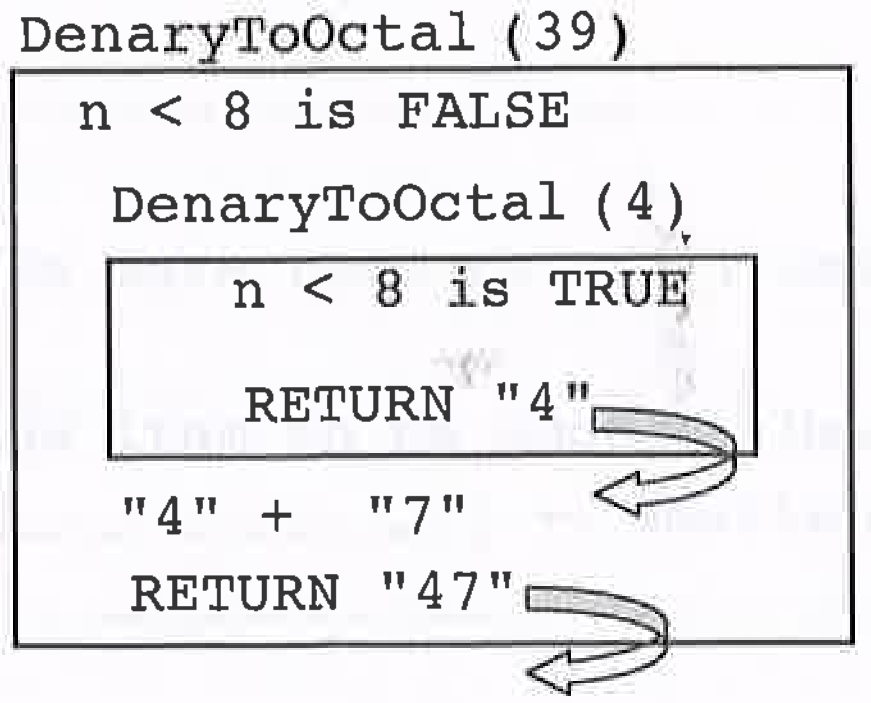
\includegraphics[width=0.5\paperwidth]{C:/Users/Admin/Desktop/Github/question_bank/LyX/static/img/9597-ALVL-2015-P2-Q4}
\par\end{center}
\begin{enumerate}
\item[(b)] Draw a similar diagram to show the execution of the call \texttt{DenaryToOctal(67)}.\hfill{}
{[}3{]}
\item[(c)] Changes are to be made to the function \texttt{DenaryToOctal()} so
that it converts denary numbers to hexadecimal.

Describe the changes: 
\begin{itemize}
\item that are essential to make the revised function work. 
\item that are non-essential but would help with the clarity of the pseudocode.\hfill{}
{[}5{]}
\end{itemize}
\end{enumerate}
{[}SPLIT\_HERE{]}
\item \textbf{{[}ALVL/9597/2015/P2/Q5{]} }

A program is to be written to test an insertion sort algorithm. A
top-down approach was used in the design of the program. The program,
\texttt{InsertionSortTester}, has a number of parts: 
\begin{itemize}
\item input integer values into the array 
\item output the initial values in the array 
\item output the sorted values in the array
\item perform the insertion sort 
\item validate the values 
\end{itemize}
\begin{enumerate}
\item Draw a diagram, which exhibits top-down design, for the \texttt{InsertionSortTester}
program. \hfill{}{[}3{]}

A list of data items is stored in the array \texttt{Values}. The pseudocode
for the insertion sort algorithm is: 

\noindent\begin{minipage}[t]{1\columnwidth}%
\texttt{01 FOR i <- 2 TO Arraysize }

\texttt{02 \qquad{}Temp <- Values{[}i{]} }

\texttt{03 \qquad{}j <- i\textemdash l }

\texttt{04 \qquad{}WHILE (j > 0) AND (Values {[}j{]} > Temp) }

\texttt{05 \qquad{}\qquad{}Values{[}j+1{]} <\textemdash{} Values
{[}j{]} }

\texttt{06 \qquad{}\qquad{}j <- j\textemdash l }

\texttt{07 \qquad{}\qquad{}ENDWHILE }

\texttt{08 \qquad{}\qquad{}Values {[}j+1{]} <- Temp }

\texttt{09 ENDFOR }%
\end{minipage}
\item The sort algorithm is to be tested using the sequence of numbers:
6, 8, 2 and 1. Copy and complete the trace table given below. 
\begin{center}
\begin{tabular}{|c|c|c|c||c|c|c|}
\hline 
\multicolumn{4}{|c||}{\texttt{Values}} &  &  & \tabularnewline
\hline 
\texttt{{[}1{]}} & \texttt{{[}2{]}} & \texttt{{[}3{]}} & \texttt{{[}4{]}} & \texttt{i} & \texttt{j} & \texttt{Temp}\tabularnewline
\hline 
\hline 
6 & 8 & 2 & 1 &  &  & \tabularnewline
\hline 
 &  &  &  &  &  & \tabularnewline
\hline 
 &  &  &  &  &  & \tabularnewline
\hline 
 &  &  &  &  &  & \tabularnewline
\hline 
 &  &  &  &  &  & \tabularnewline
\hline 
 &  &  &  &  &  & \tabularnewline
\hline 
 &  &  &  &  &  & \tabularnewline
\hline 
 &  &  &  &  &  & \tabularnewline
\hline 
 &  &  &  &  &  & \tabularnewline
\hline 
 &  &  &  &  &  & \tabularnewline
\end{tabular}
\par\end{center}

\hfill{}{[}6{]}
\item Explain why this particular algorithm is inefficient for an array
where the initial values are already in order.\hfill{} {[}2{]}
\item Give \textbf{two} different test cases for the program. Justify your
selection in each case.\hfill{} {[}4{]}
\end{enumerate}
{[}SPLIT\_HERE{]}
\item \textbf{{[}ALVL/9597/2015/P2/Q6{]} }

Students from several schools are entered for examinations in different
subjects. 

A relational database is to be used by the examination board to store
data about examination entries and results. Four tables present in
the database are STUDENT, SCHOOL, SUBJECT and STUDENT-SUBJECT.

Every time a student registers for a subject examination. a new row
is created in the STUDENT-SUBJECT table. When the result becomes available,
this is added to the appropriate row.

Each student, each school, and each subject has a unique identification
code.
\begin{enumerate}
\item {}
\begin{enumerate}
\item Draw an Entity-Relationship (E-R) diagram to show the relationship
between the STUDENT table and the SUBJECT table. \hfill{}{[}1{]}
\item State the type of relationship that exists between the STUDENT and
SUBJECT tables. \hfill{}{[}1{]}
\end{enumerate}
\item Draw an E-R diagram to show the relationship between the four tables
that provides for a fully normalised database design.\hfill{} {[}3{]}
\end{enumerate}
A table description can be expressed as: 

\texttt{TableName(Attribute1, Attribute2, Attribute3, ...)} 

The primary key is indicated by underlining one or more attributes. 

An incomplete STUDENT table is: 

\texttt{STUDENT(}\texttt{\uline{StudentID}}\texttt{, StudentName,
DateOfBirth) }
\begin{enumerate}
\item[(c)]  Give a table description for the SUBJECT table. Ensure there are
\textbf{two} attributes in addition to the primary key. \hfill{}{[}3{]}
\item[(d)]  Give a table description for the STUDENT-SUBJECT table. Ensure there
is \textbf{one} non-key attribute.\hfill{} {[}3{]}
\item[(e)] {} 
\begin{enumerate}
\item State the type of relationship that exists between the STUDENT and
the SCHOOL tables.\hfill{} {[}1{]}
\item Explain how the relationship between the STUDENT table and the SCHOOL
table is established. \hfill{}{[}3{]}
\end{enumerate}
\end{enumerate}
{[}SPLIT\_HERE{]}
\end{enumerate}

\end{document}
